\documentclass[12pt,a4paper]{article}
\usepackage[UTF8]{ctex}
\usepackage{geometry}
\geometry{left=2.5cm,right=2.5cm,top=3cm,bottom=3cm}
\usepackage{amsmath,amsfonts,amssymb}
\usepackage{graphicx}
\usepackage{booktabs}
\usepackage{multirow}
\usepackage{float}
\usepackage{hyperref}
\usepackage{cite}
\usepackage{enumerate}
\usepackage{listings}
\usepackage{xcolor}

\hypersetup{
    colorlinks=true,
    linkcolor=blue,
    filecolor=blue,
    urlcolor=blue,
    citecolor=blue
}

\title{\textbf{结合AI技术的钢铁材料性能预测研究\\\Large ——基于机器学习和深度学习的建模方法}}
\author{}
\date{\today}

\begin{document}

\maketitle

\begin{abstract}
随着人工智能技术的快速发展,其在材料科学领域的应用日益广泛。本研究基于钢卷热处理过程中的温度曲线、化学成分和性能指标数据,构建了多种机器学习模型用于性能预测。研究采用集成学习(随机森林、XGBoost、LightGBM)、支持向量回归(SVR)和深度学习(TabNet)等方法,对钢卷的抗拉强度、屈服强度和断后伸长率三个关键性能指标进行预测建模。通过5折交叉验证,结果表明XGBoost模型在三个性能指标上均表现最优,其中抗拉强度预测的R²达到0.9022。研究还通过部分依赖图(PDP)分析了关键工艺参数对性能指标的影响,为工艺优化提供了数据支持。本研究展示了AI技术在实际工业数据中的有效应用,为材料性能预测和工艺优化提供了新的思路。

\textbf{关键词:} 人工智能;机器学习;材料性能预测;钢铁材料;集成学习;深度学习
\end{abstract}

\section{引言}

材料性能预测是材料科学和工程领域的重要研究方向。传统的材料性能预测方法主要依赖于经验公式和物理模型,这些方法在面对复杂的多因素交互作用时往往存在局限性。随着大数据技术和人工智能算法的发展,基于数据驱动的机器学习方法在材料性能预测领域展现出巨大潜力。

钢铁材料作为重要的结构材料,其性能与生产工艺参数、化学成分等多因素密切相关。钢卷的热处理工艺,特别是退火工艺,对最终产品的力学性能有显著影响。传统的工艺参数优化通常依赖于专家经验和大量试验,成本高、周期长。通过建立准确的数据驱动模型,可以预测不同工艺参数组合下的材料性能,为工艺优化提供指导。

本研究以实际工业生产数据为基础,构建了完整的AI技术应用框架,包括数据预处理、特征工程、模型训练、超参数优化和结果解释等环节。研究对比了多种主流机器学习算法的性能,并通过模型解释方法分析了关键工艺参数的影响机制。

本研究的所有代码、数据和实验结果已开源,可在GitHub仓库获取:\url{https://github.com/Sellifake/Steel_Data_Analys}。

\section{研究现状分析}

\subsection{AI技术在材料科学中的应用}

人工智能技术在材料科学中的应用已得到广泛关注。机器学习方法在材料性能预测、材料设计和工艺优化等方面展现出显著优势。Chen等\cite{chen2020}综述了机器学习在材料科学中的应用,指出深度学习在复杂材料性能预测任务中表现优异。Zhang等\cite{zhang2021}使用随机森林和神经网络预测钢材的力学性能,取得了较好的预测效果。

\subsection{钢铁材料性能预测研究}

在钢铁材料性能预测领域,已有大量研究探索了不同机器学习方法的有效性。Liu等\cite{liu2019}使用支持向量回归预测高强钢的力学性能,发现核函数的选择对模型性能有重要影响。Wang等\cite{wang2020}应用梯度提升树方法预测钢板强度,强调了特征工程的重要性。近年来,深度学习方法的引入进一步提升了预测精度。Chen等\cite{chen2022}使用TabNet网络预测材料性能,展示了深度学习在表格数据建模中的潜力。

\subsection{工艺参数影响分析}

工艺参数对材料性能的影响分析是材料工程中的重要问题。传统的敏感性分析主要基于物理模型和有限元仿真,计算成本高。近年来,基于机器学习模型的部分依赖分析(PDP)和个体条件期望(ICE)方法被广泛应用于特征效应分析。这些方法能够直观地展示输入变量对输出的影响趋势,为工艺优化提供指导。

\subsection{研究现状总结}

尽管AI技术在材料性能预测领域已有广泛应用,但仍存在以下挑战:(1)实际工业数据往往存在噪声和缺失值,数据质量直接影响模型性能;(2)不同材料的性能预测需要针对性的模型设计;(3)模型可解释性不足限制了其在工程实践中的应用;(4)模型泛化能力需要在更大规模数据上验证。

本研究针对上述挑战,设计了一套完整的数据处理和建模流程,并重点考虑了模型的可解释性,通过特征重要性和PDP分析提供了工艺优化的指导。

\section{研究方法设计}

\subsection{研究总体框架}

本研究采用数据驱动的建模方法,整体流程包括数据预处理、特征工程、模型训练与优化、性能评估和结果解释五个主要环节。研究框架如图\ref{fig:framework}所示。

\begin{figure}[H]
\centering
\textbf{研究总体框架}
\begin{enumerate}
\item 数据预处理模块:从原始Excel文件中提取温度曲线数据,进行数据清洗和格式统一
\item 特征提取模块:从时间序列数据中提取35个工艺特征
\item 数据合并模块:整合工艺特征、化学成分和性能指标数据
\item 特征选择模块:基于相关性和VIF分析删除冗余特征
\item 扰动数据生成模块:生成用于敏感性分析的扰动数据集
\item 模型训练模块:训练多种机器学习模型并优化超参数
\item 模型评估模块:通过交叉验证评估模型性能
\item 结果解释模块:分析特征重要性和工艺参数影响
\end{enumerate}
\caption{研究总体框架}
\label{fig:framework}
\end{figure}

\subsection{数据来源与特征工程}

\subsubsection{数据来源}

研究数据来自实际工业生产过程,包括:
\begin{itemize}
\item \textbf{温度曲线数据}:12,737个钢卷的时间序列温度数据,包含热点和冷点两条温度曲线
\item \textbf{化学成分数据}:包含碳、硅、锰、磷、硫、铝、钛、铌、氧、氮等10种元素含量
\item \textbf{性能指标数据}:抗拉强度、屈服强度(Rp0.2值)、断后伸长率三个关键力学性能指标
\item \textbf{工艺参数数据}:退火卷宽度、冷轧入口厚度、冷轧生产实际厚度、热轧在炉时间、热轧精轧入口/出口平均温度、热轧卷取平均温度等7个额外工艺特征
\end{itemize}

\subsubsection{特征提取}

从温度曲线中提取了35个工艺特征,主要包括:
\begin{enumerate}
\item \textbf{温度特征}:热点和冷点的峰值温度
\item \textbf{时间特征}:升温时长、保温时长、降温时长
\item \textbf{速率特征}:升温速率、降温速率及其标准差、最大瞬时速率
\item \textbf{温度变化特征}:升温幅度、降温幅度、保温阶段温降
\item \textbf{温度差异特征}:热点与冷点之间的峰值温度差、平均温度差、速率差等
\end{enumerate}

此外,研究还计算了"压下率"这一衍生特征,定义为:
\begin{equation}
\text{压下率} = \frac{\text{冷轧入口厚度} - \text{冷轧生产实际厚度}}{\text{冷轧入口厚度}}
\end{equation}

\subsubsection{数据清洗与预处理}

数据预处理包括以下步骤:
\begin{enumerate}
\item \textbf{缺失值处理}:删除目标变量缺失的记录;对工艺特征中的缺失值使用中位数填充
\item \textbf{异常值处理}:删除冷点峰值温度为0的记录;删除化学成分全部为0或全部缺失的记录
\item \textbf{数据类型转换}:将所有特征和指标强制转换为数值类型,无法转换的值标记为NaN后删除
\item \textbf{数据去重}:基于钢卷号去除重复记录
\end{enumerate}

经过预处理,从原始的12,737个钢卷数据中,提取出3,250条唯一工艺记录,最终合并性能数据后得到2,760条有效样本。

\subsection{特征选择}

研究采用相关性分析和方差膨胀因子(VIF)分析进行特征选择:
\begin{enumerate}
\item \textbf{相关性分析}:计算所有特征之间的Pearson相关系数,识别高度相关的特征对
\item \textbf{VIF分析}:计算输入特征(工艺特征和化学成分)的方差膨胀因子,识别多重共线性问题
\item \textbf{特征删除}:根据领域知识和统计分析,删除了43个冗余特征,最终保留35个输入特征
\end{enumerate}

最终数据集包含2,760行样本,39列特征(35个输入特征 + 3个性能指标 + 1个ID列)。

\subsection{机器学习模型设计}

研究采用五种主流机器学习方法构建预测模型:

\subsubsection{集成学习方法}

\textbf{1. 随机森林(Random Forest)}

随机森林是一种基于决策树的集成学习方法,通过构建多棵决策树并取其平均值来提高预测精度和模型稳定性。模型参数设置为:n\_estimators=100,使用5折交叉验证评估性能。

\textbf{2. XGBoost(eXtreme Gradient Boosting)}

XGBoost是一种梯度提升框架,通过迭代优化逐步提升模型性能。研究使用RandomizedSearchCV进行超参数调优,搜索参数包括:
\begin{itemize}
\item n\_estimators: 100-1200
\item learning\_rate: 0.01-0.2
\item max\_depth: 3-12
\item subsample: 0.6-1.0
\item colsample\_bytree: 0.6-1.0
\item gamma: 0-0.5
\item reg\_alpha: 0-1 (L1正则化)
\item reg\_lambda: 0-1 (L2正则化)
\end{itemize}

共进行200次迭代搜索,使用R²作为优化目标。

\textbf{3. LightGBM(Light Gradient Boosting Machine)}

LightGBM是一种高效的梯度提升框架,使用基于梯度的单侧采样和互斥特征捆绑技术加速训练。超参数调优策略与XGBoost类似,主要包括:n\_estimators、learning\_rate、max\_depth、num\_leaves、subsample、colsample\_bytree、reg\_alpha、reg\_lambda等参数。

\subsubsection{支持向量回归(SVR)}

使用RBF核函数的支持向量回归模型处理非线性关系。通过Pipeline将StandardScaler和SVR组合,确保数据标准化。使用RandomizedSearchCV对C参数(0.1-1000,对数均匀分布)和gamma参数(0.0001-0.1,对数均匀分布)进行50次迭代搜索。

\subsubsection{深度学习模型(TabNet)}

TabNet是专门为表格数据设计的神经网络架构,具有内置的注意力机制,能够自动学习特征重要性。研究使用Optuna进行贝叶斯超参数优化,优化目标为5折交叉验证的R²均值。TabNet的优势在于其可解释性,通过注意力权重提供特征重要性分析。

\subsection{模型评估方法}

所有模型均采用5折交叉验证进行评估,评估指标包括:
\begin{itemize}
\item \textbf{R²分数}(决定系数):衡量模型解释方差的能力,取值0-1,越接近1越好
\item \textbf{MAE}(平均绝对误差):衡量预测值与真实值的平均偏差
\item \textbf{RMSE}(均方根误差):对较大误差更加敏感的综合误差指标
\end{itemize}

\subsection{模型解释与结果分析}

\subsubsection{特征重要性分析}

对于树模型(随机森林、XGBoost、LightGBM),使用模型内置的特征重要性计算方法;对于SVR,使用排列重要性(Permutation Importance)方法;对于TabNet,直接提取其内置的特征重要性权重。

\subsubsection{部分依赖图(PDP)分析}

为了分析关键工艺参数对性能指标的影响,研究生成扰动数据集:
\begin{itemize}
\item \textbf{热点峰值温度}:在原始值基础上从-10°C到+10°C变化,步长1°C(21个扰动点)
\item \textbf{冷点峰值温度}:在原始值基础上从-10°C到+10°C变化,步长1°C(21个扰动点)
\item \textbf{保温时长}:在原始值基础上从-3600秒到+3600秒变化,步长60秒(121个扰动点)
\end{itemize}

对每个原始样本生成多个扰动变体,共生成449,880个扰动样本。使用训练好的模型对所有扰动样本进行预测,然后计算部分依赖图(PDP),展示扰动参数对性能指标的期望影响,并计算95\%置信区间。

\section{实验结果与分析}

\subsection{数据处理结果}

经过完整的数据处理流程,最终得到的数据集统计如下:
\begin{itemize}
\item 原始数据:12,737个钢卷的时间序列数据
\item 工艺特征提取后:3,250条唯一工艺记录
\item 合并性能数据后:2,760行有效样本
\item 特征选择后:39列(35个输入特征 + 3个性能指标 + 1个ID列)
\end{itemize}

相关性分析显示,部分工艺特征与性能指标存在显著相关性,如峰值温度与抗拉强度、保温时长与屈服强度等。VIF分析表明,经过特征选择后,输入特征的多重共线性问题得到有效控制。

\subsection{模型性能对比}

表\ref{tab:performance}展示了五种模型在三个性能指标上的预测性能。

\begin{table}[H]
\centering
\caption{各模型性能对比(R²分数)}
\label{tab:performance}
\begin{tabular}{lccc}
\toprule
模型 & 抗拉强度 & 屈服Rp0.2值* & 断后伸长率 \\
\midrule
随机森林 & 0.8991 & 0.7670 & 0.5044 \\
XGBoost & \textbf{0.9022} & \textbf{0.7766} & \textbf{0.5194} \\
LightGBM & 0.8962 & 0.7655 & 0.5120 \\
SVR & 0.8908 & 0.7347 & 0.4593 \\
TabNet & 0.8512 & 0.6820 & 0.3895 \\
\bottomrule
\end{tabular}
\end{table}

图\ref{fig:model_comparison}展示了五种机器学习模型在预测三个性能指标(抗拉强度、屈服Rp0.2值、断后伸长率)时的综合性能对比。该图包含九个子图,分别展示了每个性能指标对应的R²分数、平均绝对误差(MAE)和均方根误差(RMSE)三个评估指标。从图中可以清晰看出,XGBoost模型在所有指标上均表现最优,特别是在抗拉强度预测中,R²达到0.9022,MAE为7.26,RMSE为10.32。集成学习方法(随机森林、XGBoost、LightGBM)整体表现优于支持向量回归和TabNet神经网络,验证了集成学习在处理材料性能预测问题时的优势。

\begin{figure}[H]
\centering
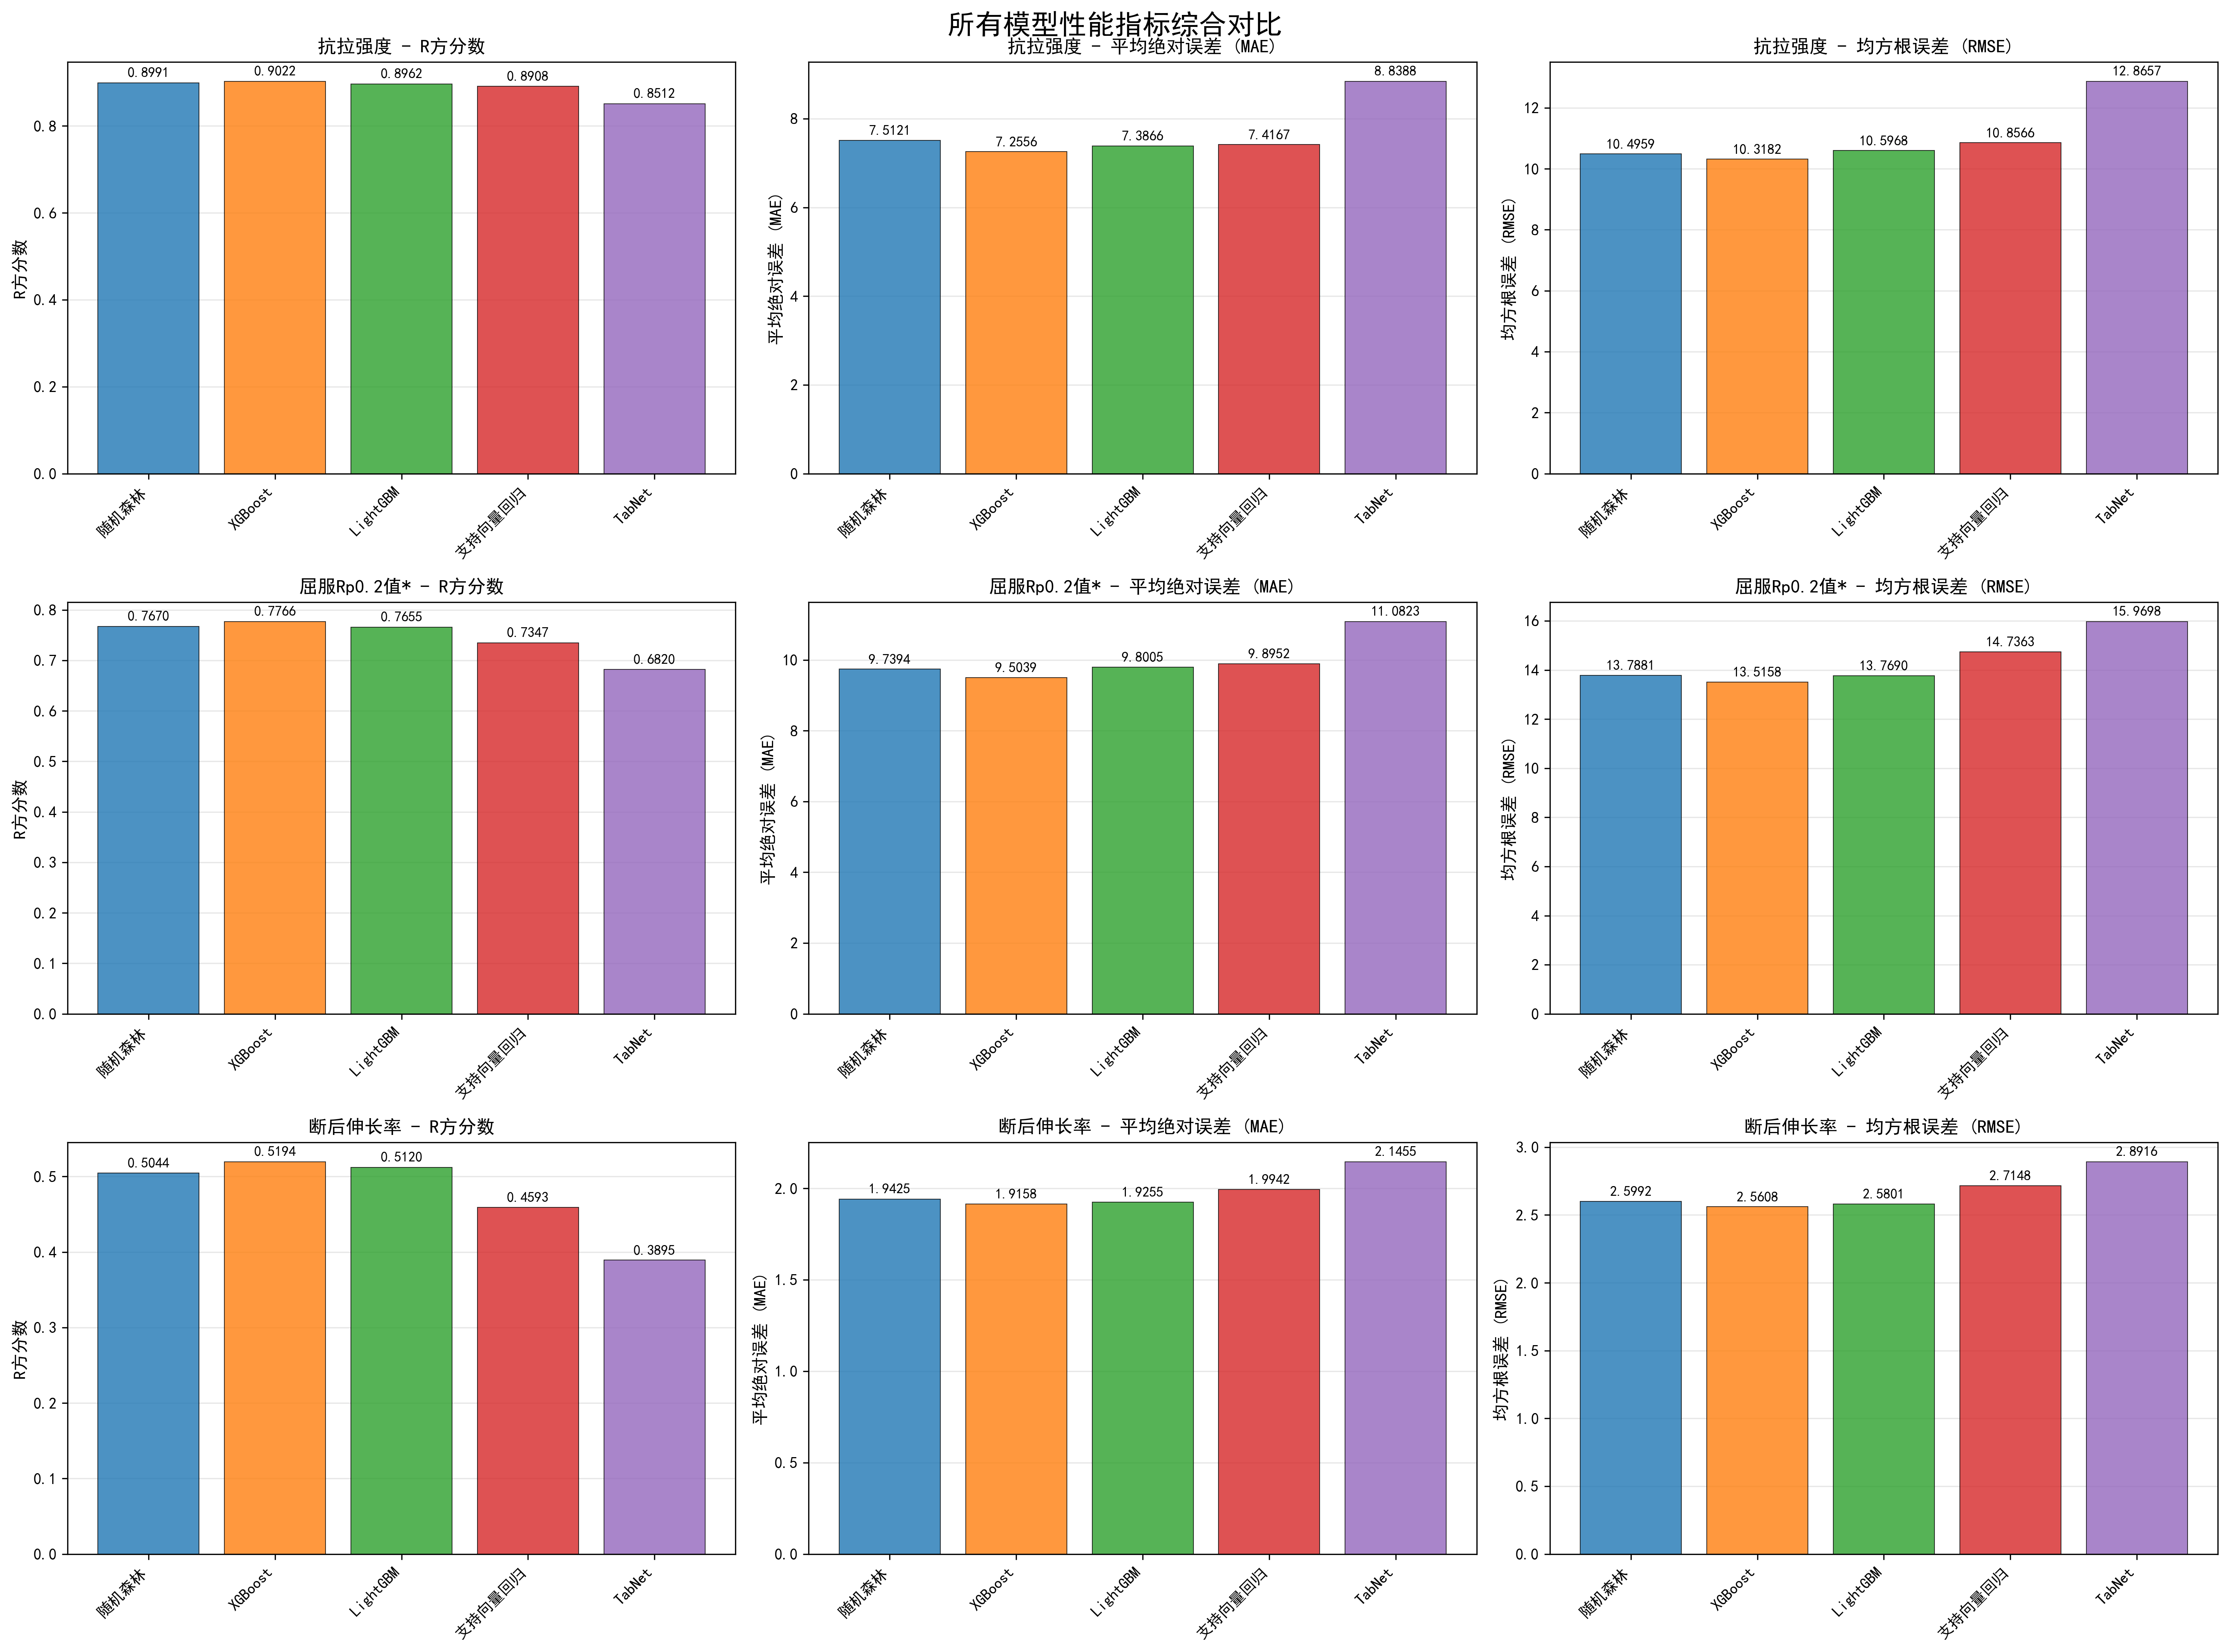
\includegraphics[width=0.95\textwidth]{fig/01_comprehensive_model_performance_comparison.png}
\caption{各模型性能综合对比图。图中展示了五种模型(随机森林、XGBoost、LightGBM、SVR、TabNet)在三个性能指标(抗拉强度、屈服Rp0.2值、断后伸长率)上的R²分数、MAE和RMSE表现。每个性能指标对应一行,每个评估指标对应一列,共九个子图。}
\label{fig:model_comparison}
\end{figure}

从表\ref{tab:performance}可以看出:

\textbf{1. 抗拉强度预测}

XGBoost模型表现最优(R²=0.9022),表明抗拉强度与输入特征之间存在较强的非线性关系,梯度提升算法能够有效捕捉这些关系。随机森林和LightGBM也取得了较好效果(R²>0.89),说明集成学习方法在处理此类问题上具有优势。SVR和TabNet的表现相对较差,可能与数据规模和模型复杂度有关。

\textbf{2. 屈服强度预测}

XGBoost同样表现最优(R²=0.7766),但相比抗拉强度,预测精度有所下降,说明屈服强度的预测难度更大,可能受到更多随机因素的影响。所有树模型(随机森林、XGBoost、LightGBM)的性能相近,都超过了0.76,而SVR和TabNet的表现明显较差。

\textbf{3. 断后伸长率预测}

这是三个指标中预测难度最大的,最佳模型XGBoost的R²仅为0.5194。这可能是因为断后伸长率受到更多微观组织因素的影响,而本研究主要关注宏观工艺参数。尽管如此,集成学习方法仍明显优于SVR和TabNet。

\subsection{详细性能指标}

表\ref{tab:detailed_performance}展示了XGBoost模型(表现最优)在三个指标上的详细性能。

\begin{table}[H]
\centering
\caption{XGBoost模型详细性能指标}
\label{tab:detailed_performance}
\begin{tabular}{lccc}
\toprule
性能指标 & R² & MAE & RMSE \\
\midrule
抗拉强度 & 0.9022 & 7.26 & 10.32 \\
屈服Rp0.2值* & 0.7766 & 9.50 & 13.52 \\
断后伸长率 & 0.5194 & 1.92 & 2.56 \\
\bottomrule
\end{tabular}
\end{table}

\subsection{特征重要性分析}

通过对XGBoost模型的特征重要性分析,发现以下关键特征对性能预测贡献最大:

\textbf{对抗拉强度影响最大的特征:}
\begin{enumerate}
\item 热点峰值温度
\item 冷点峰值温度
\item 保温时长
\item 冷点升温幅度
\item 热点保温温度标准差
\end{enumerate}

\textbf{对屈服强度影响最大的特征:}
\begin{enumerate}
\item 热点峰值温度
\item 冷点峰值温度
\item 保温时长
\item 热点降温幅度
\item 冷点平均降温速率
\end{enumerate}

\textbf{对断后伸长率影响最大的特征:}
\begin{enumerate}
\item 保温时长
\item 热点峰值温度
\item 冷点峰值温度
\item 冷点保温温度标准差
\item 压下率
\end{enumerate}

可以看出,峰值温度(热点和冷点)和保温时长是最重要的工艺参数,这与材料科学的理论认知一致。温度和时间是影响材料组织转变和性能的关键因素。

图\ref{fig:feature_freq_duanhou}、图\ref{fig:feature_freq_kangla}和图\ref{fig:feature_freq_qufu}分别展示了三个性能指标的特征重要性频率分析结果。这些图表通过统计不同模型中被识别为重要特征的出现频率,揭示了各特征在性能预测中的稳定性。

图\ref{fig:feature_freq_duanhou}展示了断后伸长率的特征重要性频率分析。图表分为左右两部分,左侧展示"前5重要特征",右侧展示"后5重要特征"。从图中可以看出,碳含量和硅含量出现频率最高(各3次),是最常被识别为前5重要特征的因素;锰含量、压下率和冷点峰值温度各出现2次,也具有较高的重要性频率。

\begin{figure}[H]
\centering
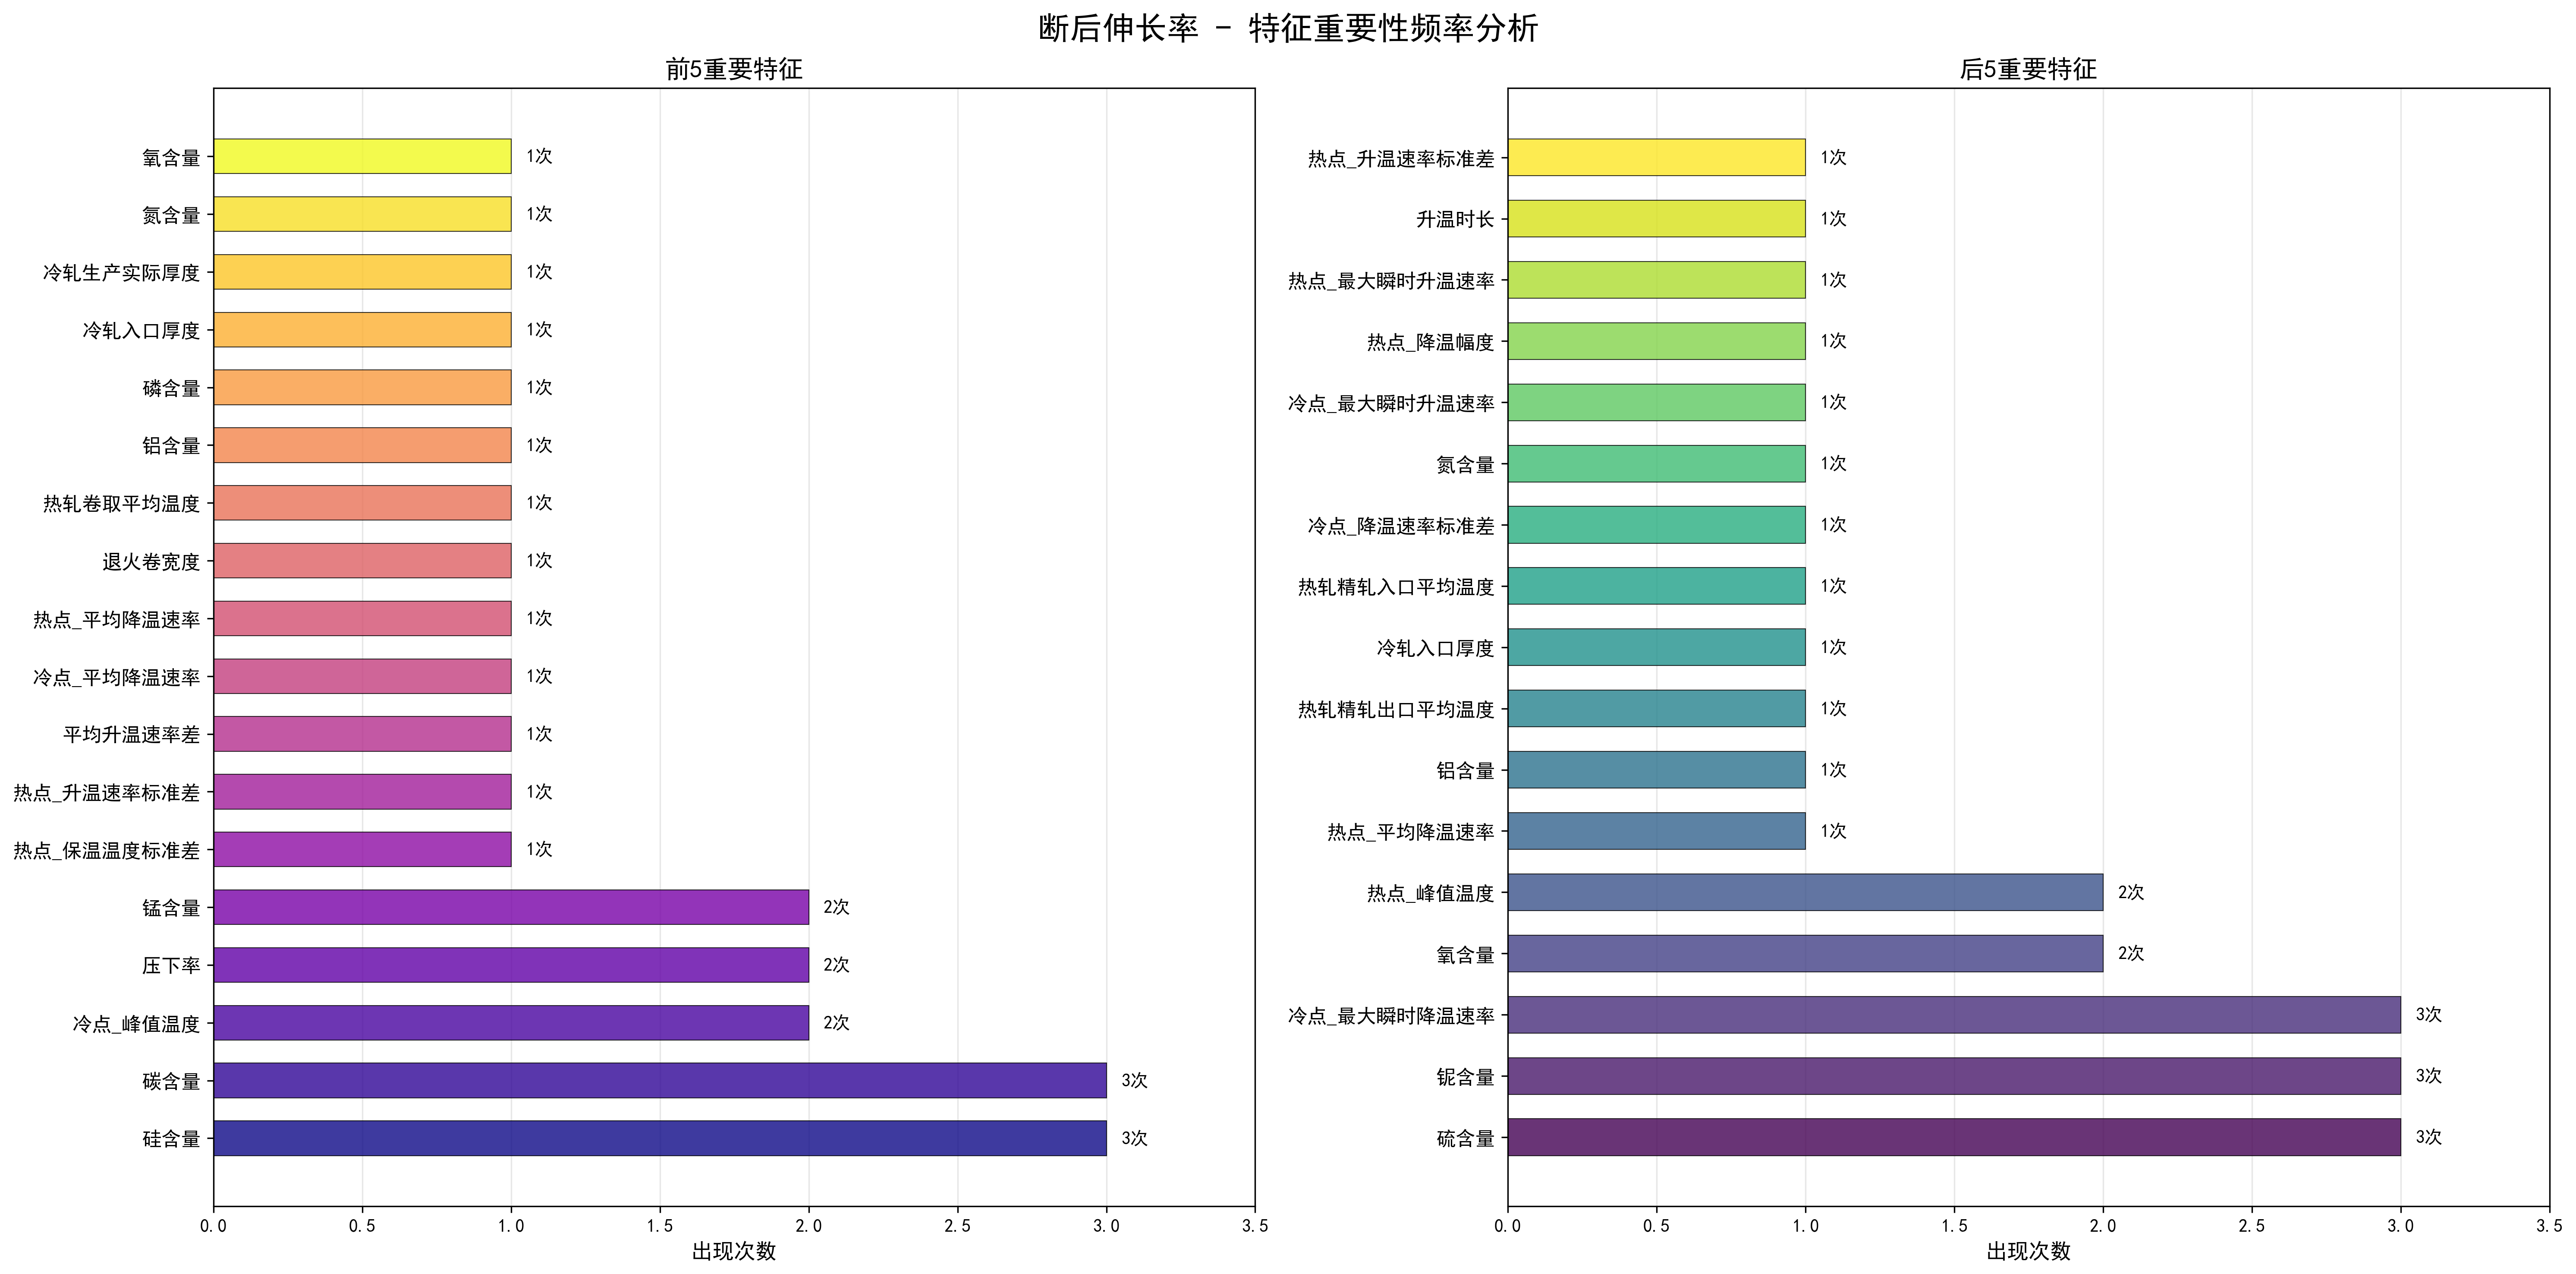
\includegraphics[width=0.95\textwidth]{fig/feature_frequency_analysis_elongation.png}
\caption{断后伸长率特征重要性频率分析。左图为"前5重要特征"出现频率,右图为"后5重要特征"出现频率。横轴表示特征在不同模型中被识别为重要特征的次数,纵轴列出各特征名称。颜色从黄色(低频)到深蓝色(高频)渐变,直观展示各特征的重要性稳定性。}
\label{fig:feature_freq_duanhou}
\end{figure}

图\ref{fig:feature_freq_kangla}展示了抗拉强度的特征重要性频率分析。左侧"前5重要特征"中,碳含量出现频率最高(4次),是预测抗拉强度最重要的因素;磷含量、硅含量和锰含量各出现3次,也具有较高的重要性;氮含量和压下率各出现2次。右侧"后5重要特征"中,热点降温幅度和铌含量出现频率较高(各3次)。这一结果与材料科学理论一致,表明化学成分,特别是碳含量,对抗拉强度具有决定性影响。

\begin{figure}[H]
\centering
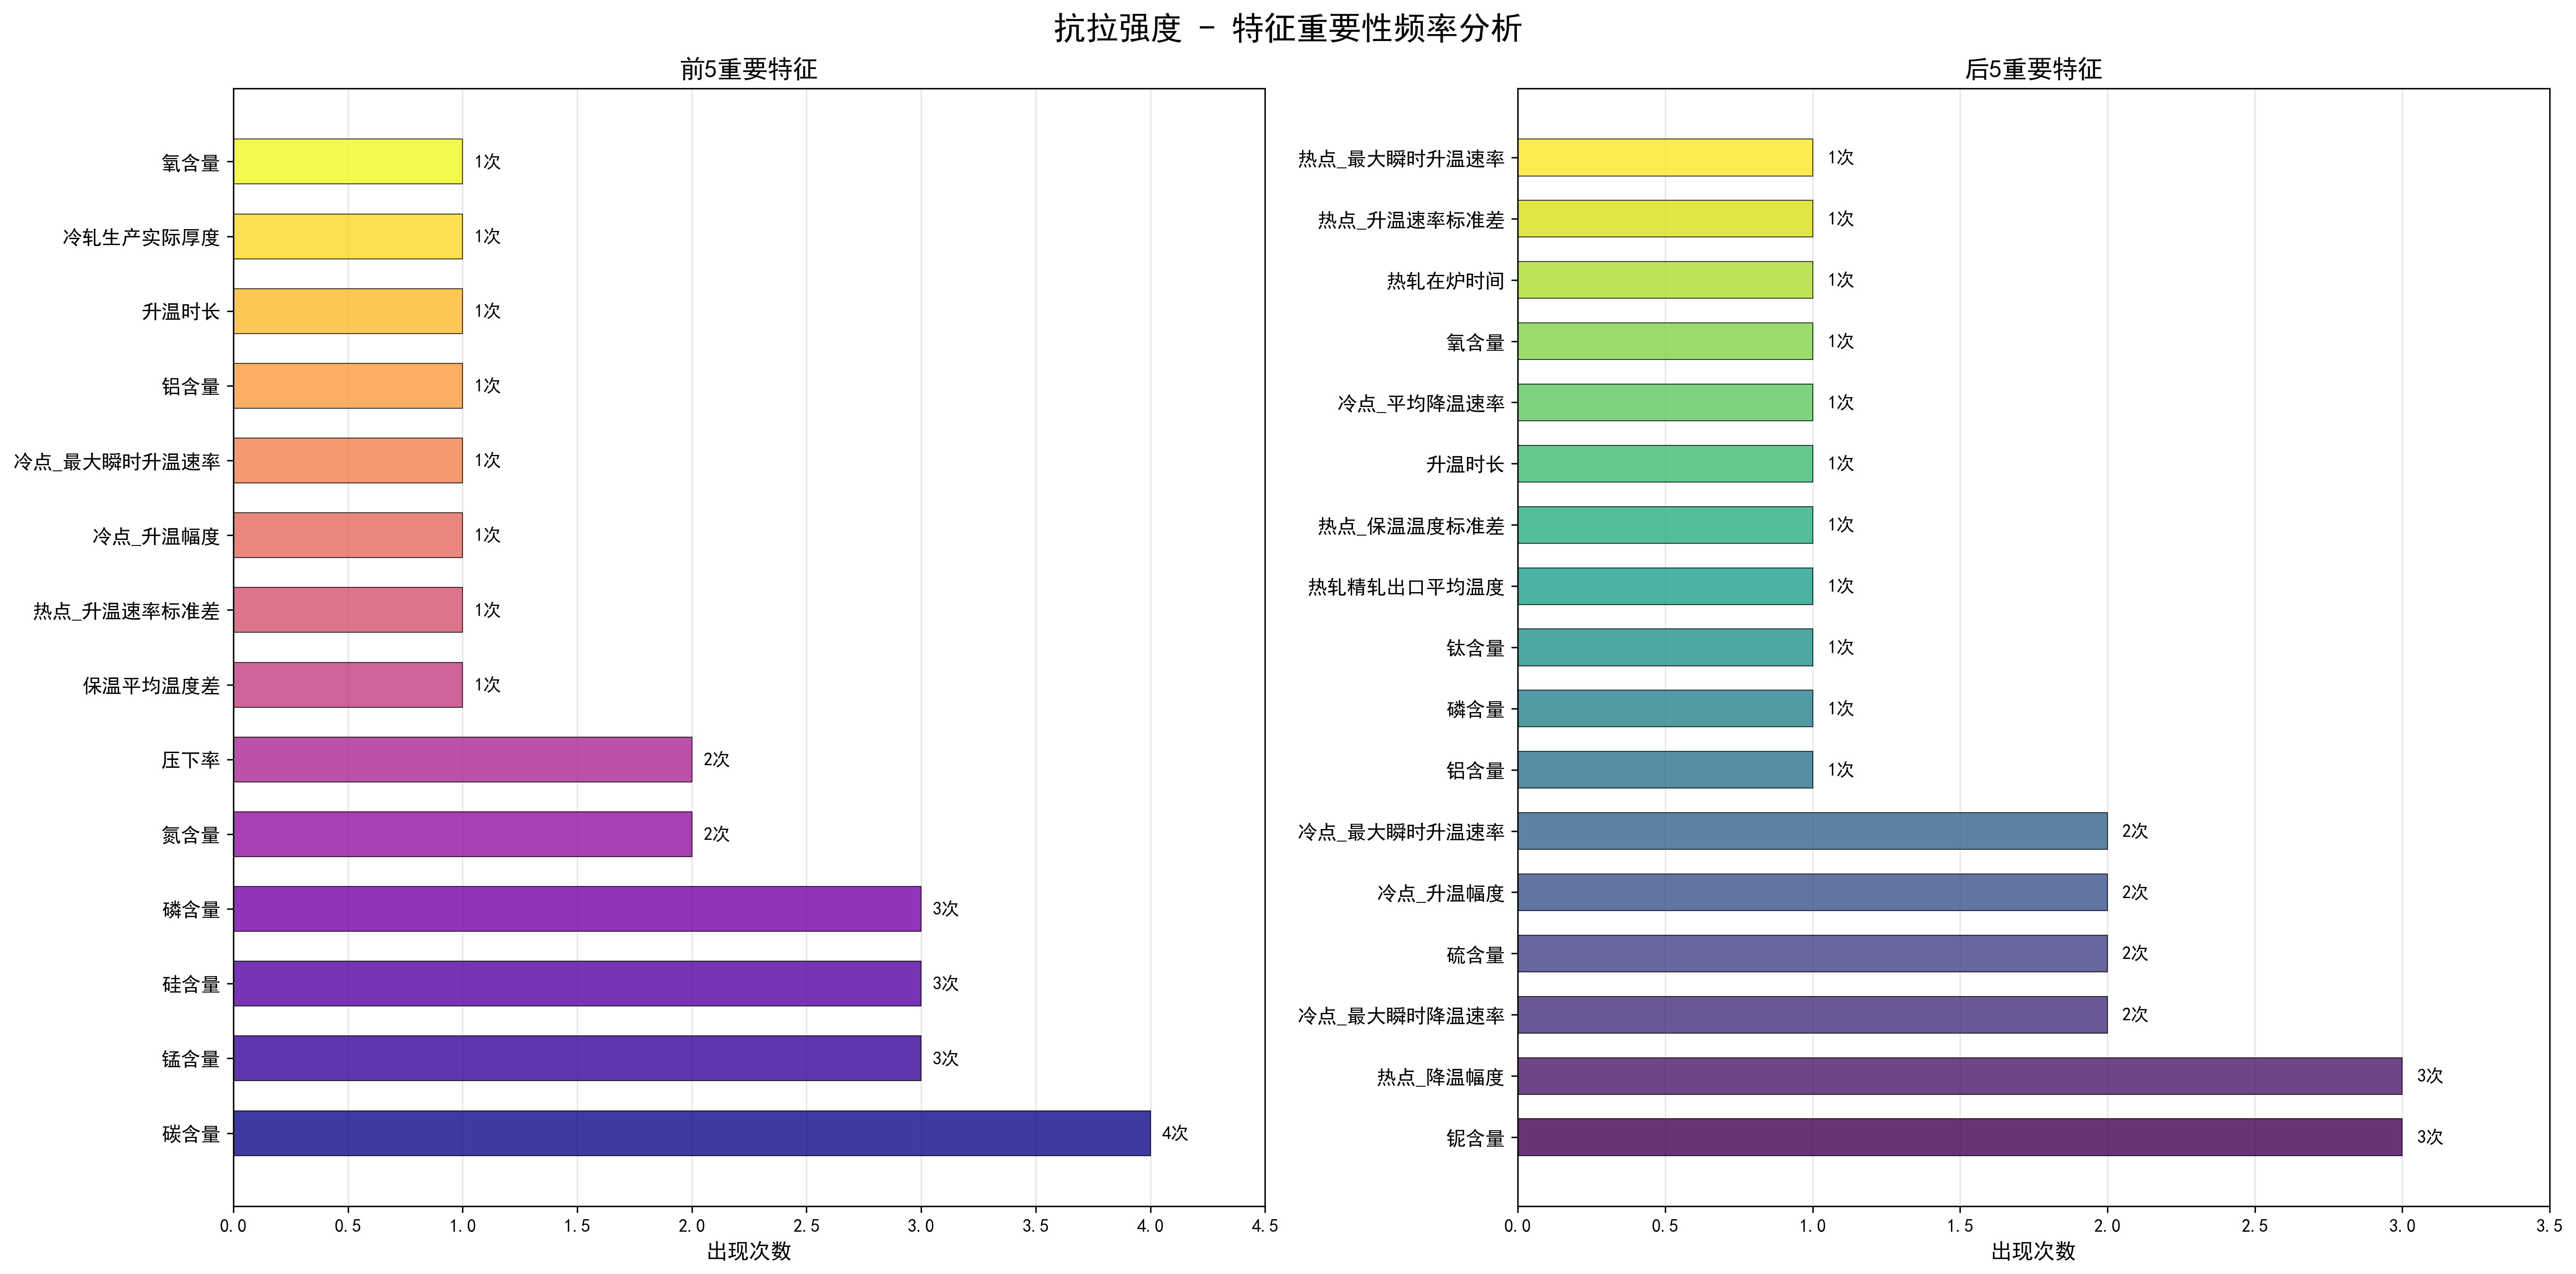
\includegraphics[width=0.95\textwidth]{fig/feature_frequency_analysis_tensile_strength.png}
\caption{抗拉强度特征重要性频率分析。左图为"前5重要特征"出现频率,右图为"后5重要特征"出现频率。从图中可以看出,碳含量是出现频率最高的特征(4次),其次是磷含量、硅含量和锰含量(各3次),说明这些化学成分对抗拉强度预测具有关键作用。}
\label{fig:feature_freq_kangla}
\end{figure}

图\ref{fig:feature_freq_qufu}展示了屈服Rp0.2值的特征重要性频率分析。左侧"前5重要特征"中,碳含量出现频率最高(5次),是所有性能指标中出现频率最高的特征,进一步证明了碳含量对钢材性能的关键作用;锰含量、氮含量和硅含量各出现3次,升温时长出现2次。右侧"后5重要特征"中,冷点最大瞬时升温速率和冷点最大瞬时降温速率出现频率较高(各4次),说明降温过程的剧烈程度对屈服强度也有一定影响。

\begin{figure}[H]
\centering
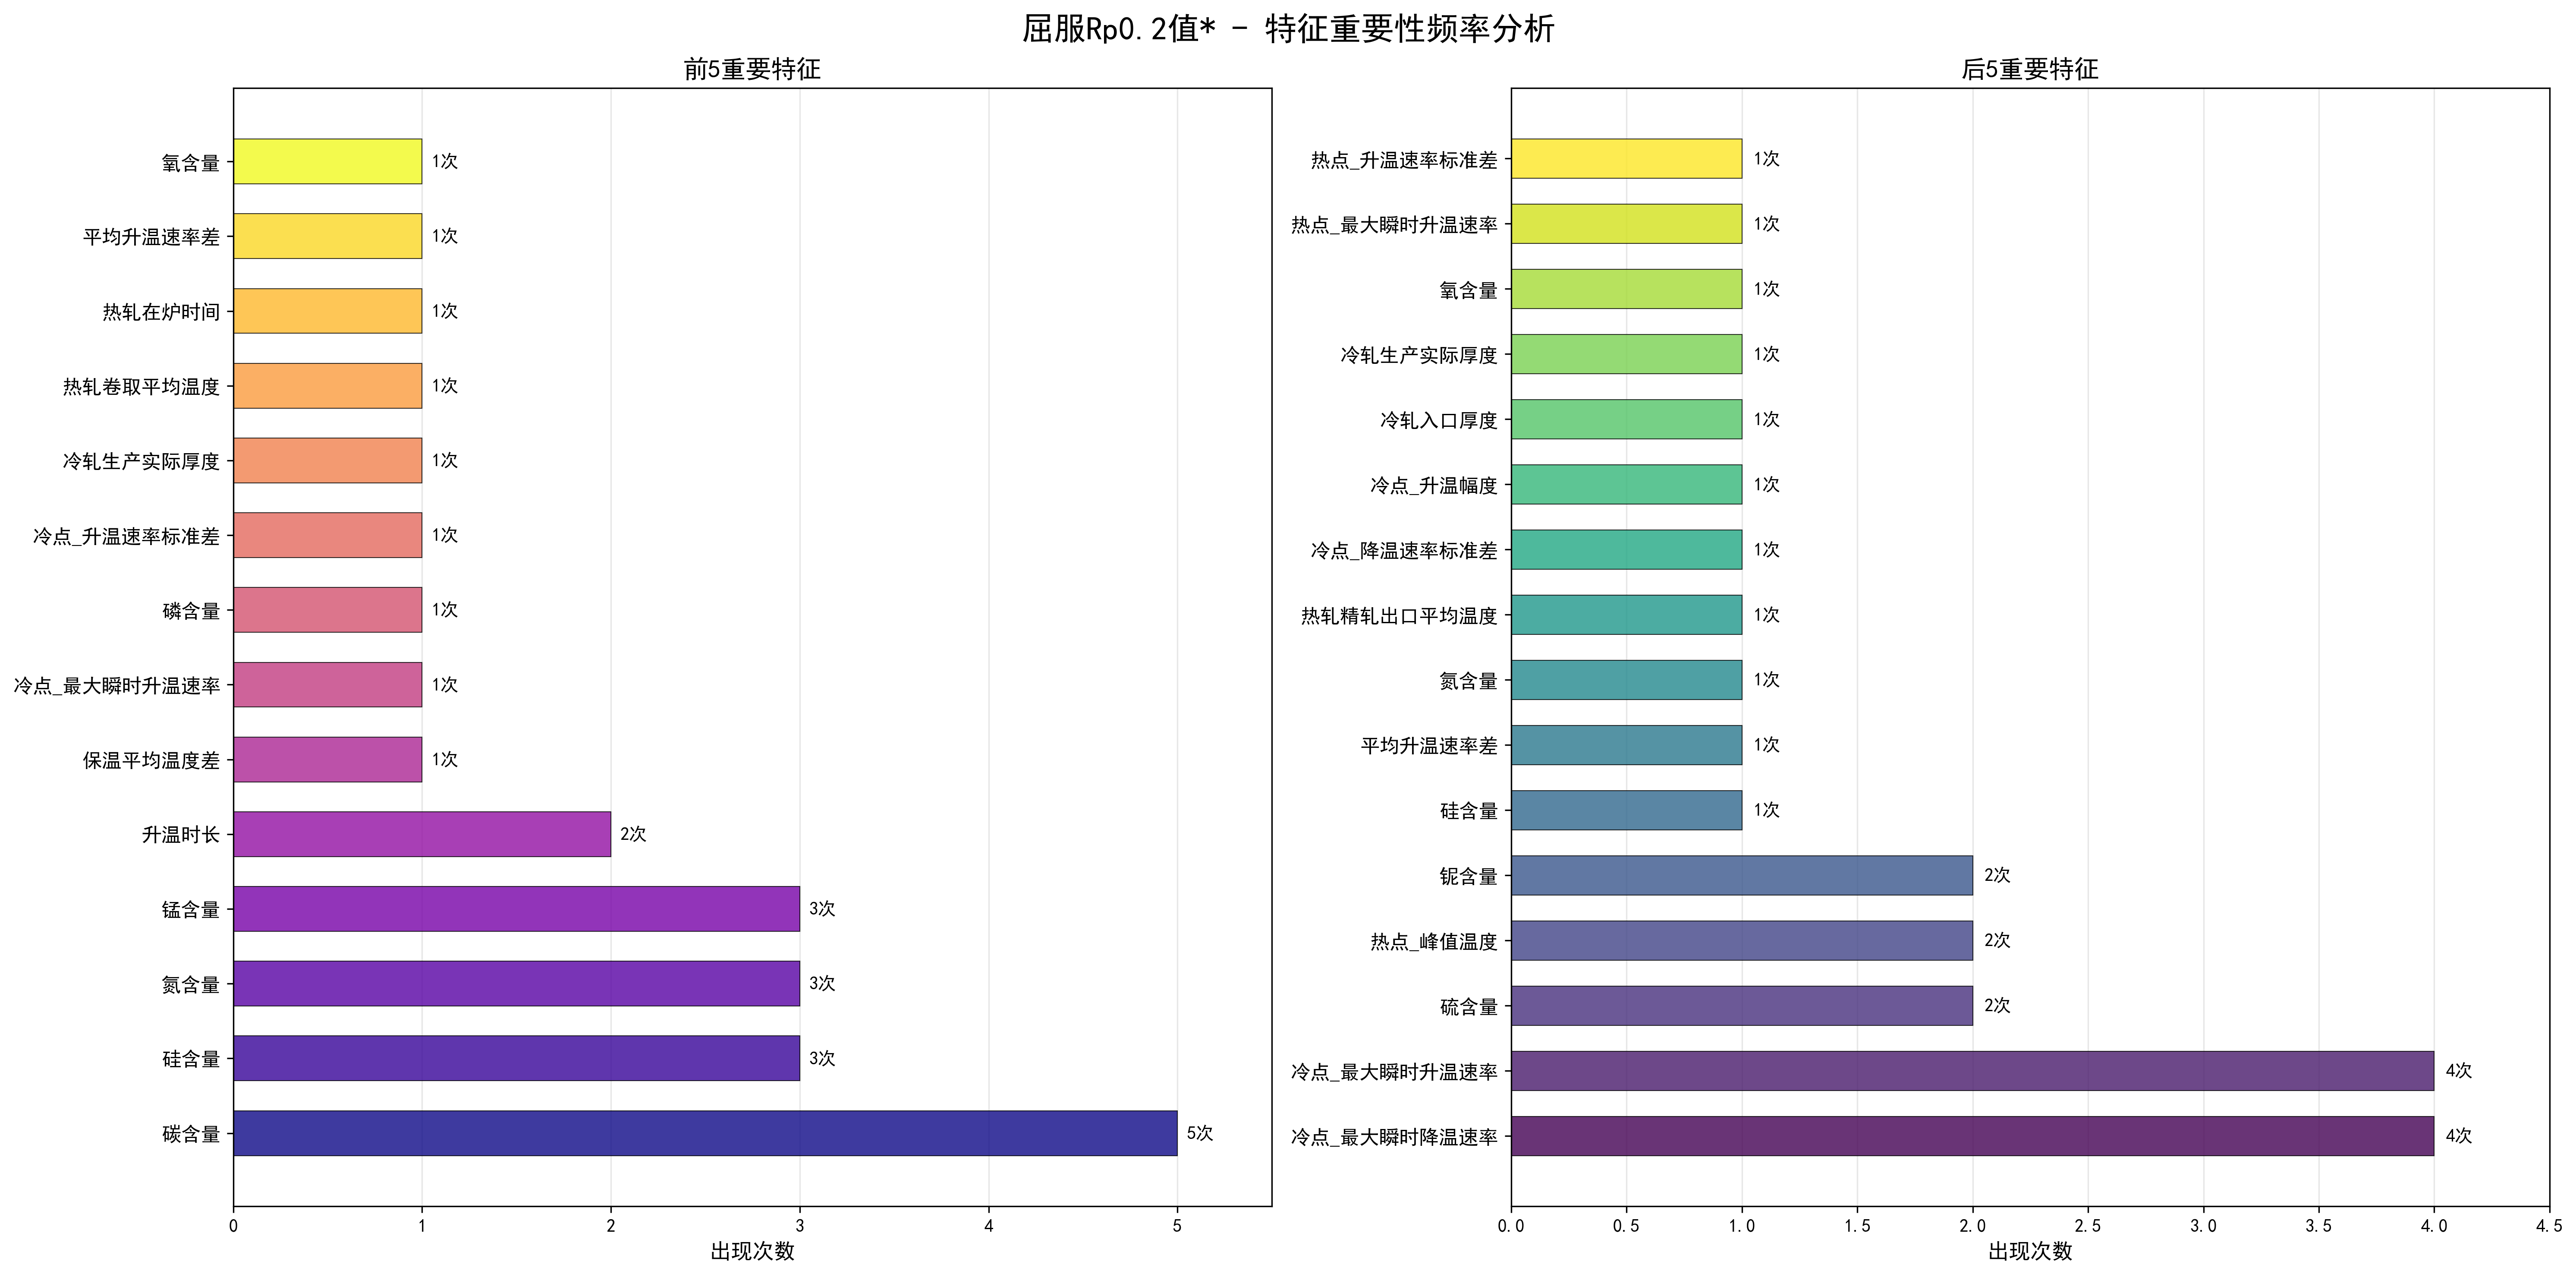
\includegraphics[width=0.95\textwidth]{fig/feature_frequency_analysis_yield_strength.png}
\caption{屈服Rp0.2值特征重要性频率分析。左图为"前5重要特征"出现频率,右图为"后5重要特征"出现频率。碳含量出现频率达到5次,是所有特征中频率最高的,表明碳含量对屈服强度具有决定性影响。锰含量、氮含量和硅含量也表现出较高的重要性(各3次)。}
\label{fig:feature_freq_qufu}
\end{figure}

从以上特征重要性频率分析可以看出,不同性能指标的关键特征存在明显差异。对于断后伸长率,碳含量和硅含量出现频率最高(各3次),是预测断后伸长率最稳定的重要特征;锰含量、压下率和冷点峰值温度各出现2次,说明这些特征也具有较高的重要性稳定性。对于抗拉强度,碳含量出现频率最高(4次),是预测抗拉强度最关键的单一因素;磷含量、硅含量和锰含量各出现3次,共同构成了预测抗拉强度的核心特征集。对于屈服强度,碳含量出现频率达到5次,是所有分析中出现频率最高的特征,充分说明了碳含量对钢材屈服强度的决定性作用。



综合以上特征重要性分析,可以得出以下结论:(1)化学成分,特别是碳、锰、硅、磷、氮等主要合金元素,是影响钢材性能的最关键因素;(2)工艺参数中,峰值温度和保温时长等温度时间参数也具有重要作用;(3)不同性能指标的特征重要性模式存在差异,抗拉强度和屈服强度主要受化学成分影响,而断后伸长率还受到工艺参数如压下率的影响。这些发现为材料设计和工艺优化提供了重要指导。

\subsection{工艺参数影响分析}

通过PDP分析,研究揭示了关键工艺参数对性能指标的影响趋势。图\ref{fig:pdp_baowen}、图\ref{fig:pdp_lengdian}和图\ref{fig:pdp_redian}分别展示了保温时长、冷点峰值温度和热点峰值温度对抗拉强度的影响。

\textbf{1. 保温时长的影响}

图\ref{fig:pdp_baowen}展示了保温时长扰动值对抗拉强度的影响。从图中可以看出,在-3000到+3000秒的扰动范围内,预测的抗拉强度均值几乎保持水平,稳定在约325左右,表明保温时长的变化对抗拉强度影响较小。95\%置信区间也非常狭窄,说明预测值稳定且不确定性低。这可能意味着在当前工艺参数范围内,保温时长的微小变化对最终抗拉强度影响有限,或者其影响已被其他更重要的特征所主导。

\begin{figure}[H]
\centering
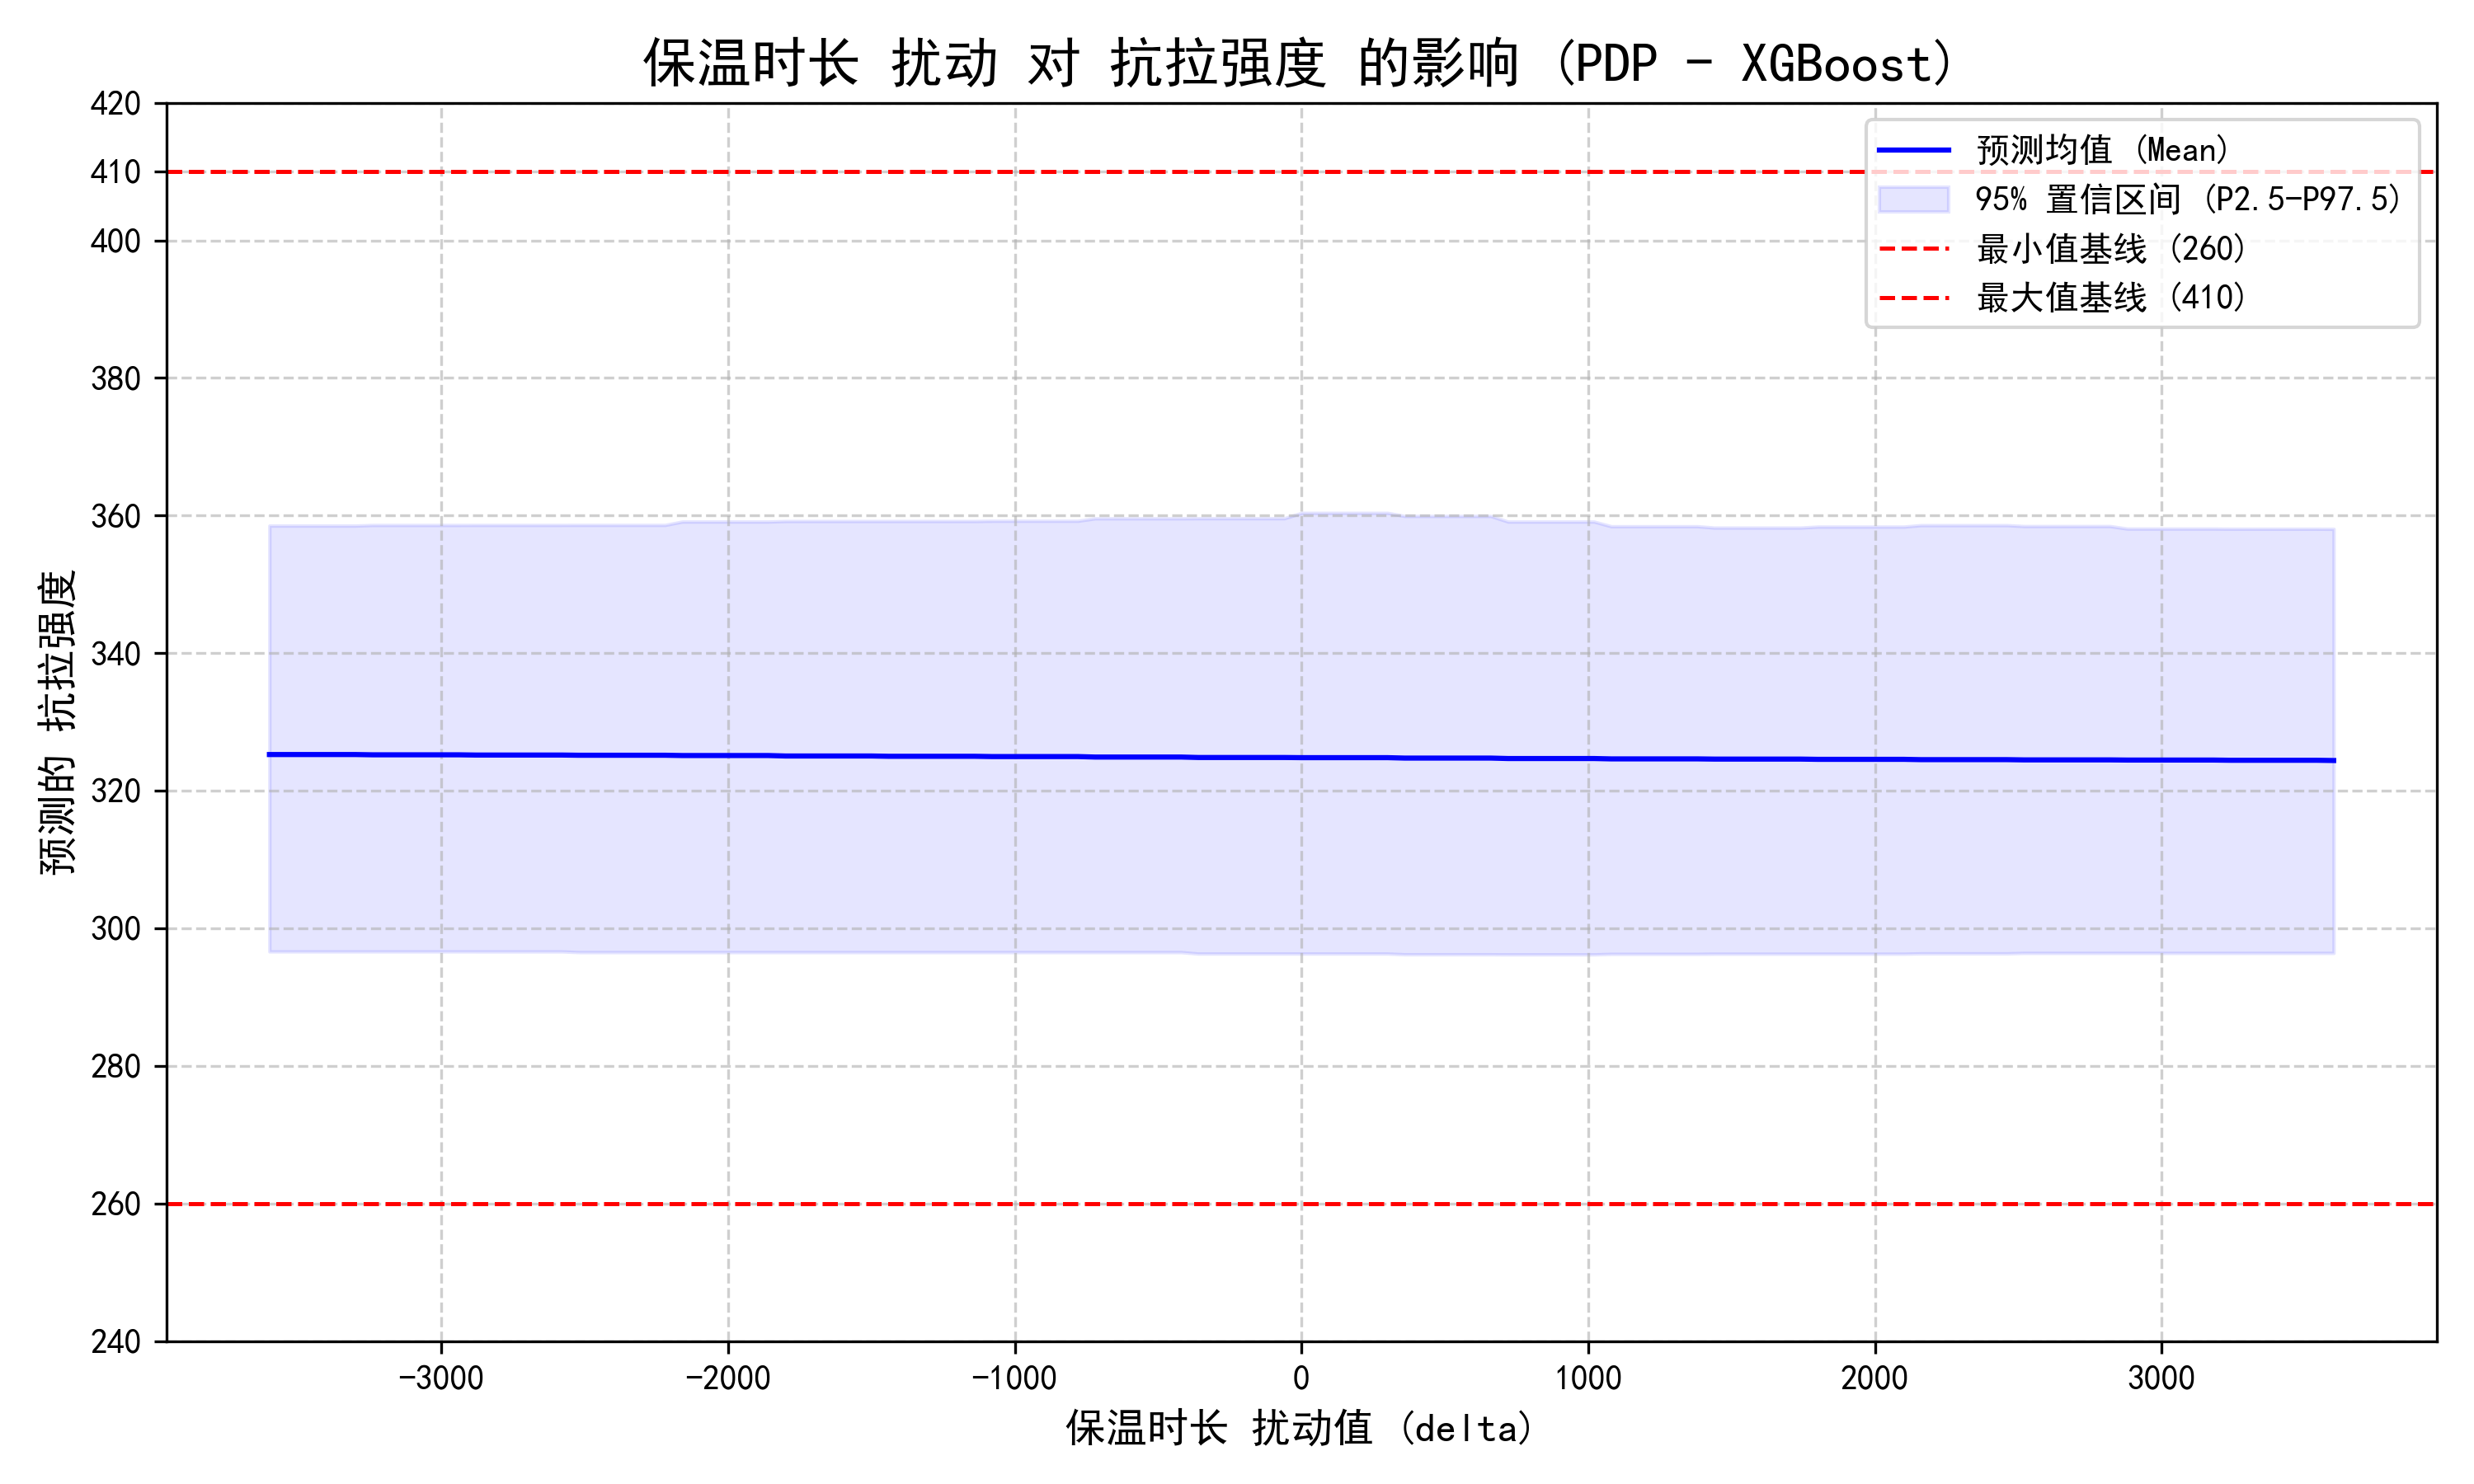
\includegraphics[width=0.75\textwidth]{fig/02b_pdp_plot_holding_time_vs_tensile_strength.png}
\caption{保温时长扰动对抗拉强度影响的PDP图(基于XGBoost模型)。X轴表示保温时长扰动值(delta),范围为-3000到3000秒;Y轴表示预测的抗拉强度,范围为240到420。蓝色实线为预测均值,浅蓝色阴影区域为95\%置信区间,红色虚线分别表示最小值基线(260)和最大值基线(410)。}
\label{fig:pdp_baowen}
\end{figure}

\textbf{2. 冷点峰值温度的影响}

图\ref{fig:pdp_lengdian}展示了冷点峰值温度扰动值对抗拉强度的影响。图中显示,在-10°C到+10°C的扰动范围内,预测的抗拉强度均值保持在320-325之间,几乎呈水平线,表明冷点峰值温度的微小变化对抗拉强度预测均值几乎没有影响。95\%置信区间相对稳定,覆盖约295到360的范围。这一结果说明冷点峰值温度在当前模型中并非对抗拉强度有显著影响的关键特征,其变化对预测的抗拉强度均值没有表现出明显的正向或负向趋势。

\begin{figure}[H]
\centering
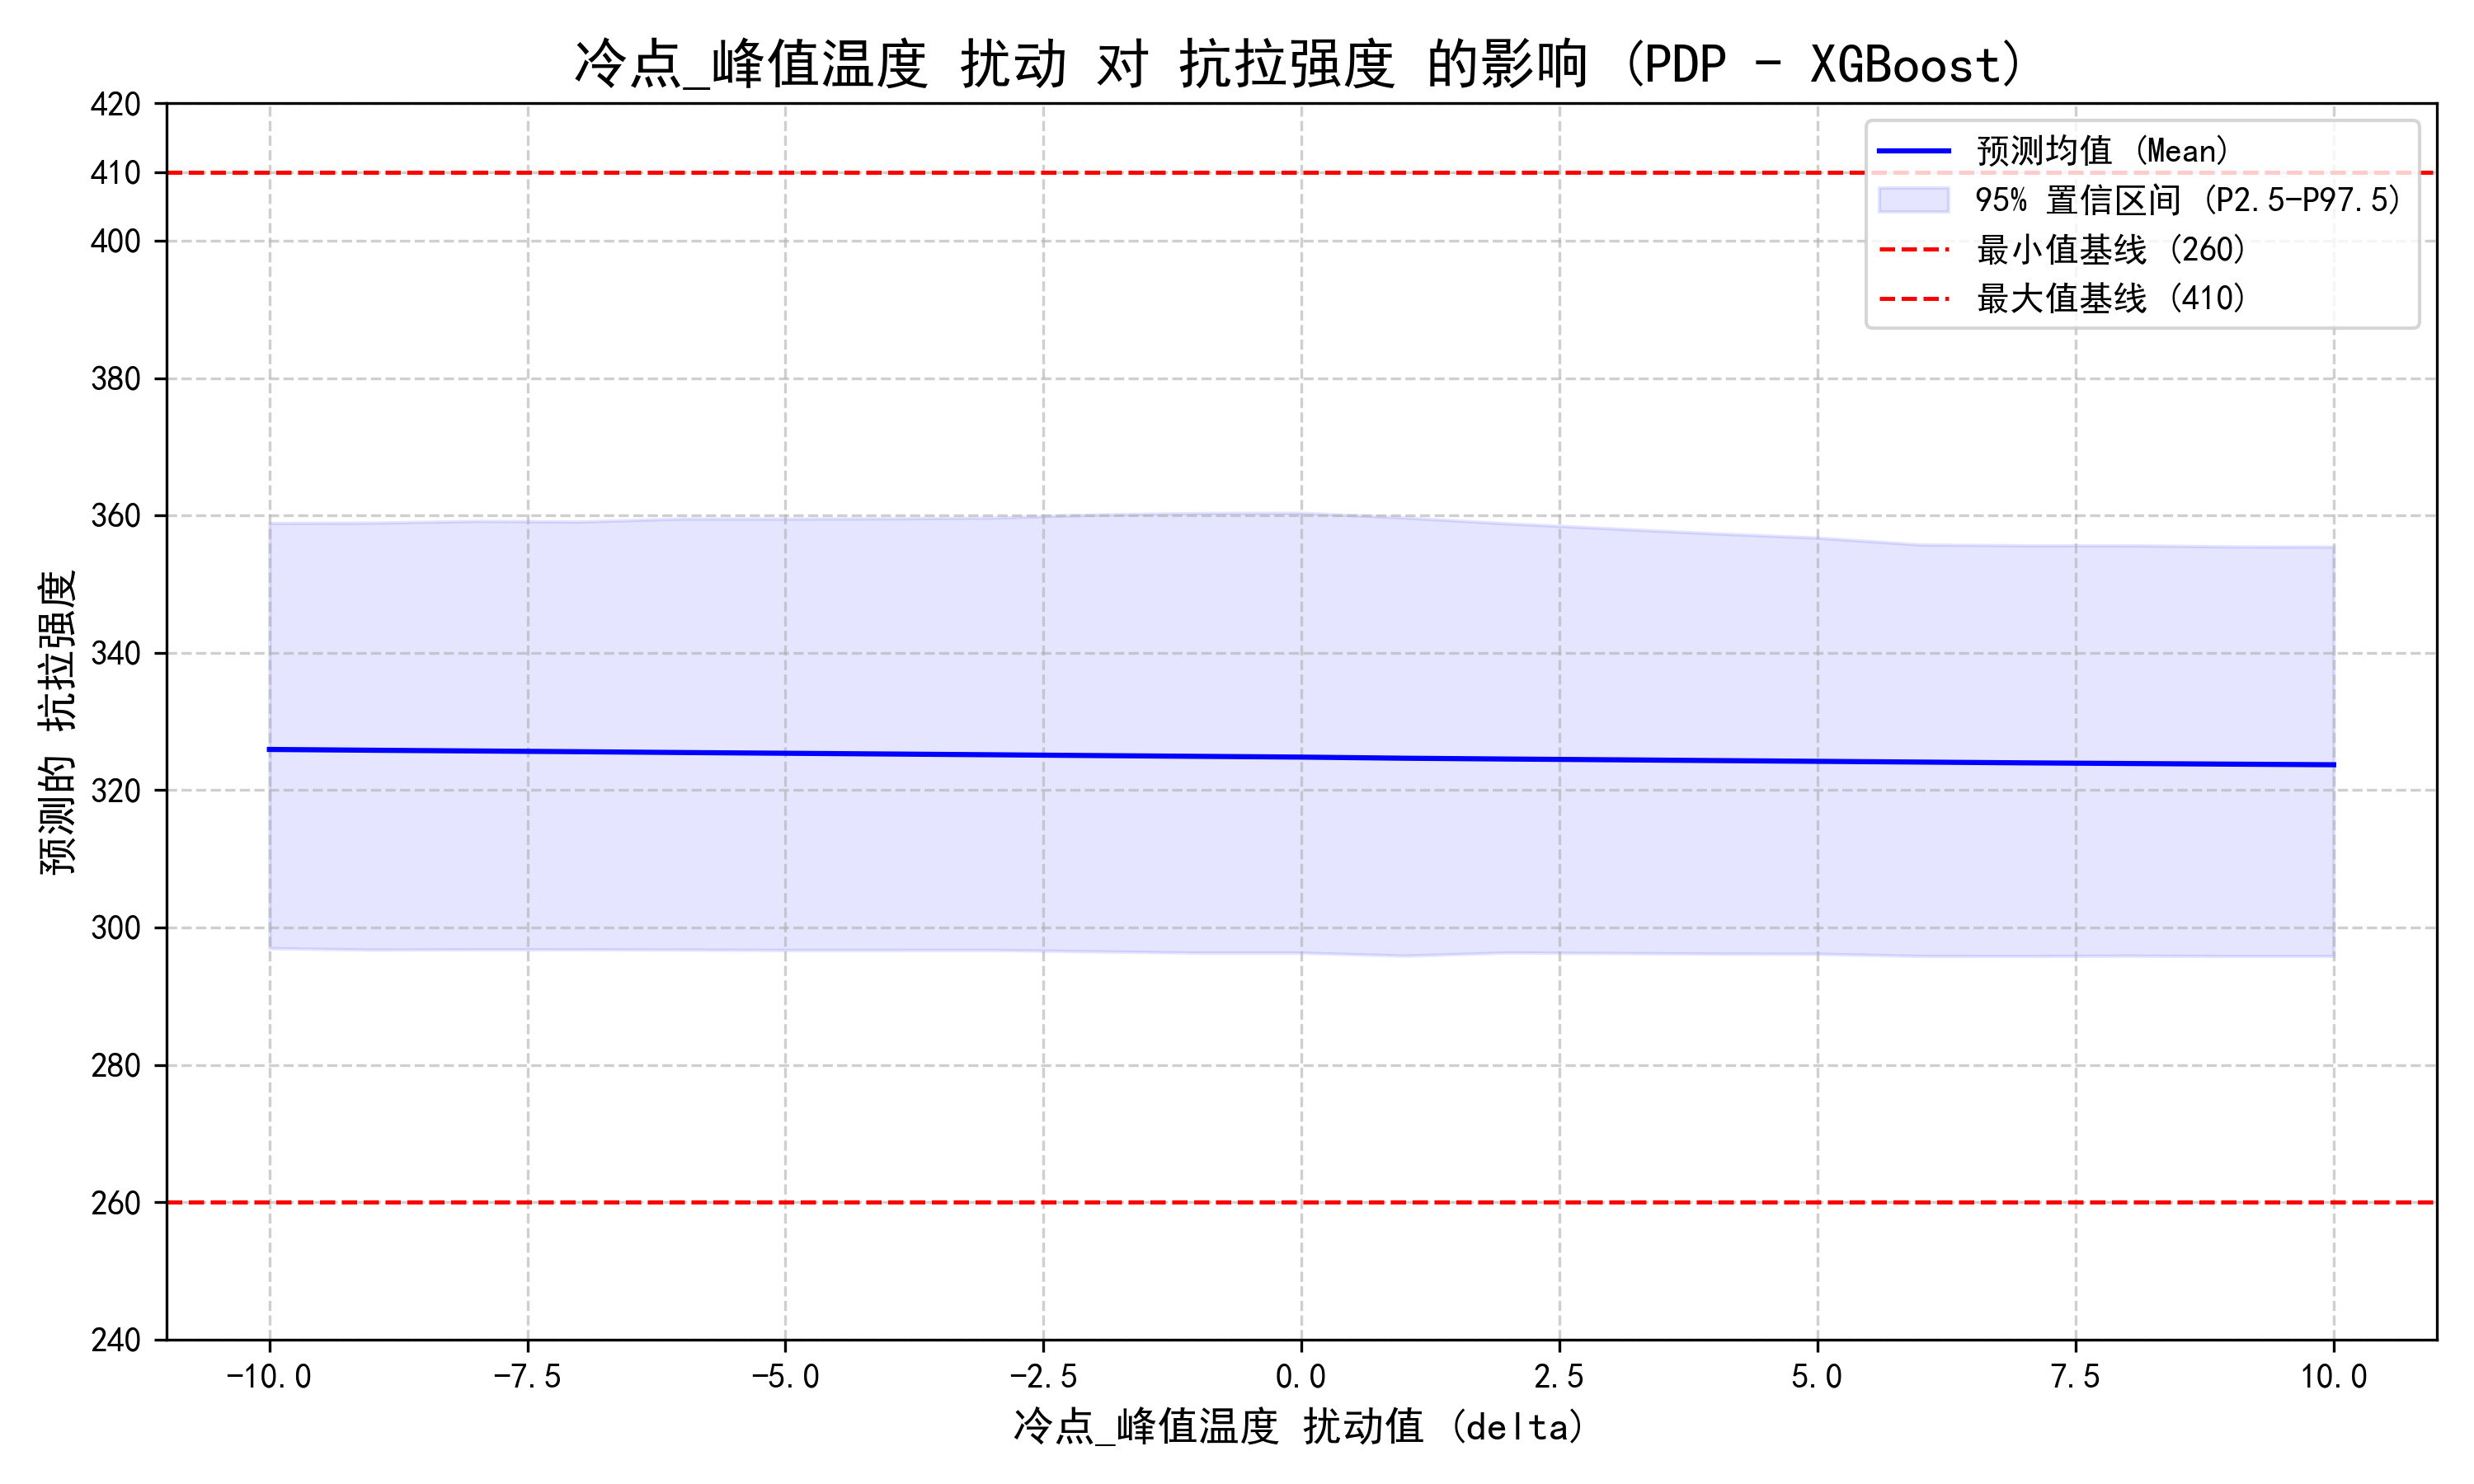
\includegraphics[width=0.75\textwidth]{fig/02b_pdp_plot_cold_spot_temp_vs_tensile_strength.png}
\caption{冷点峰值温度扰动对抗拉强度影响的PDP图(基于XGBoost模型)。X轴表示冷点峰值温度扰动值(delta),范围为-10.0到10.0°C;Y轴表示预测的抗拉强度,范围为240到420。蓝色实线为预测均值,浅蓝色阴影区域为95\%置信区间,红色虚线分别表示最小值基线(260)和最大值基线(410)。}
\label{fig:pdp_lengdian}
\end{figure}

\textbf{3. 热点峰值温度的影响}

图\ref{fig:pdp_redian}展示了热点峰值温度扰动值对抗拉强度的影响。与冷点峰值温度类似,在-10°C到+10°C的扰动范围内,预测的抗拉强度均值稳定在323-324左右,呈水平趋势,表明热点峰值温度的微小扰动对抗拉强度预测均值没有显著影响。95\%置信区间保持平坦且宽度一致,大约从295延伸到360。这说明在XGBoost模型中,热点峰值温度在较小扰动范围内对抗拉强度的影响不明显,可能因为扰动范围较小不足以引起性能指标的显著波动,或者该特征的影响在模型中被其他特征所掩盖。

\begin{figure}[H]
\centering
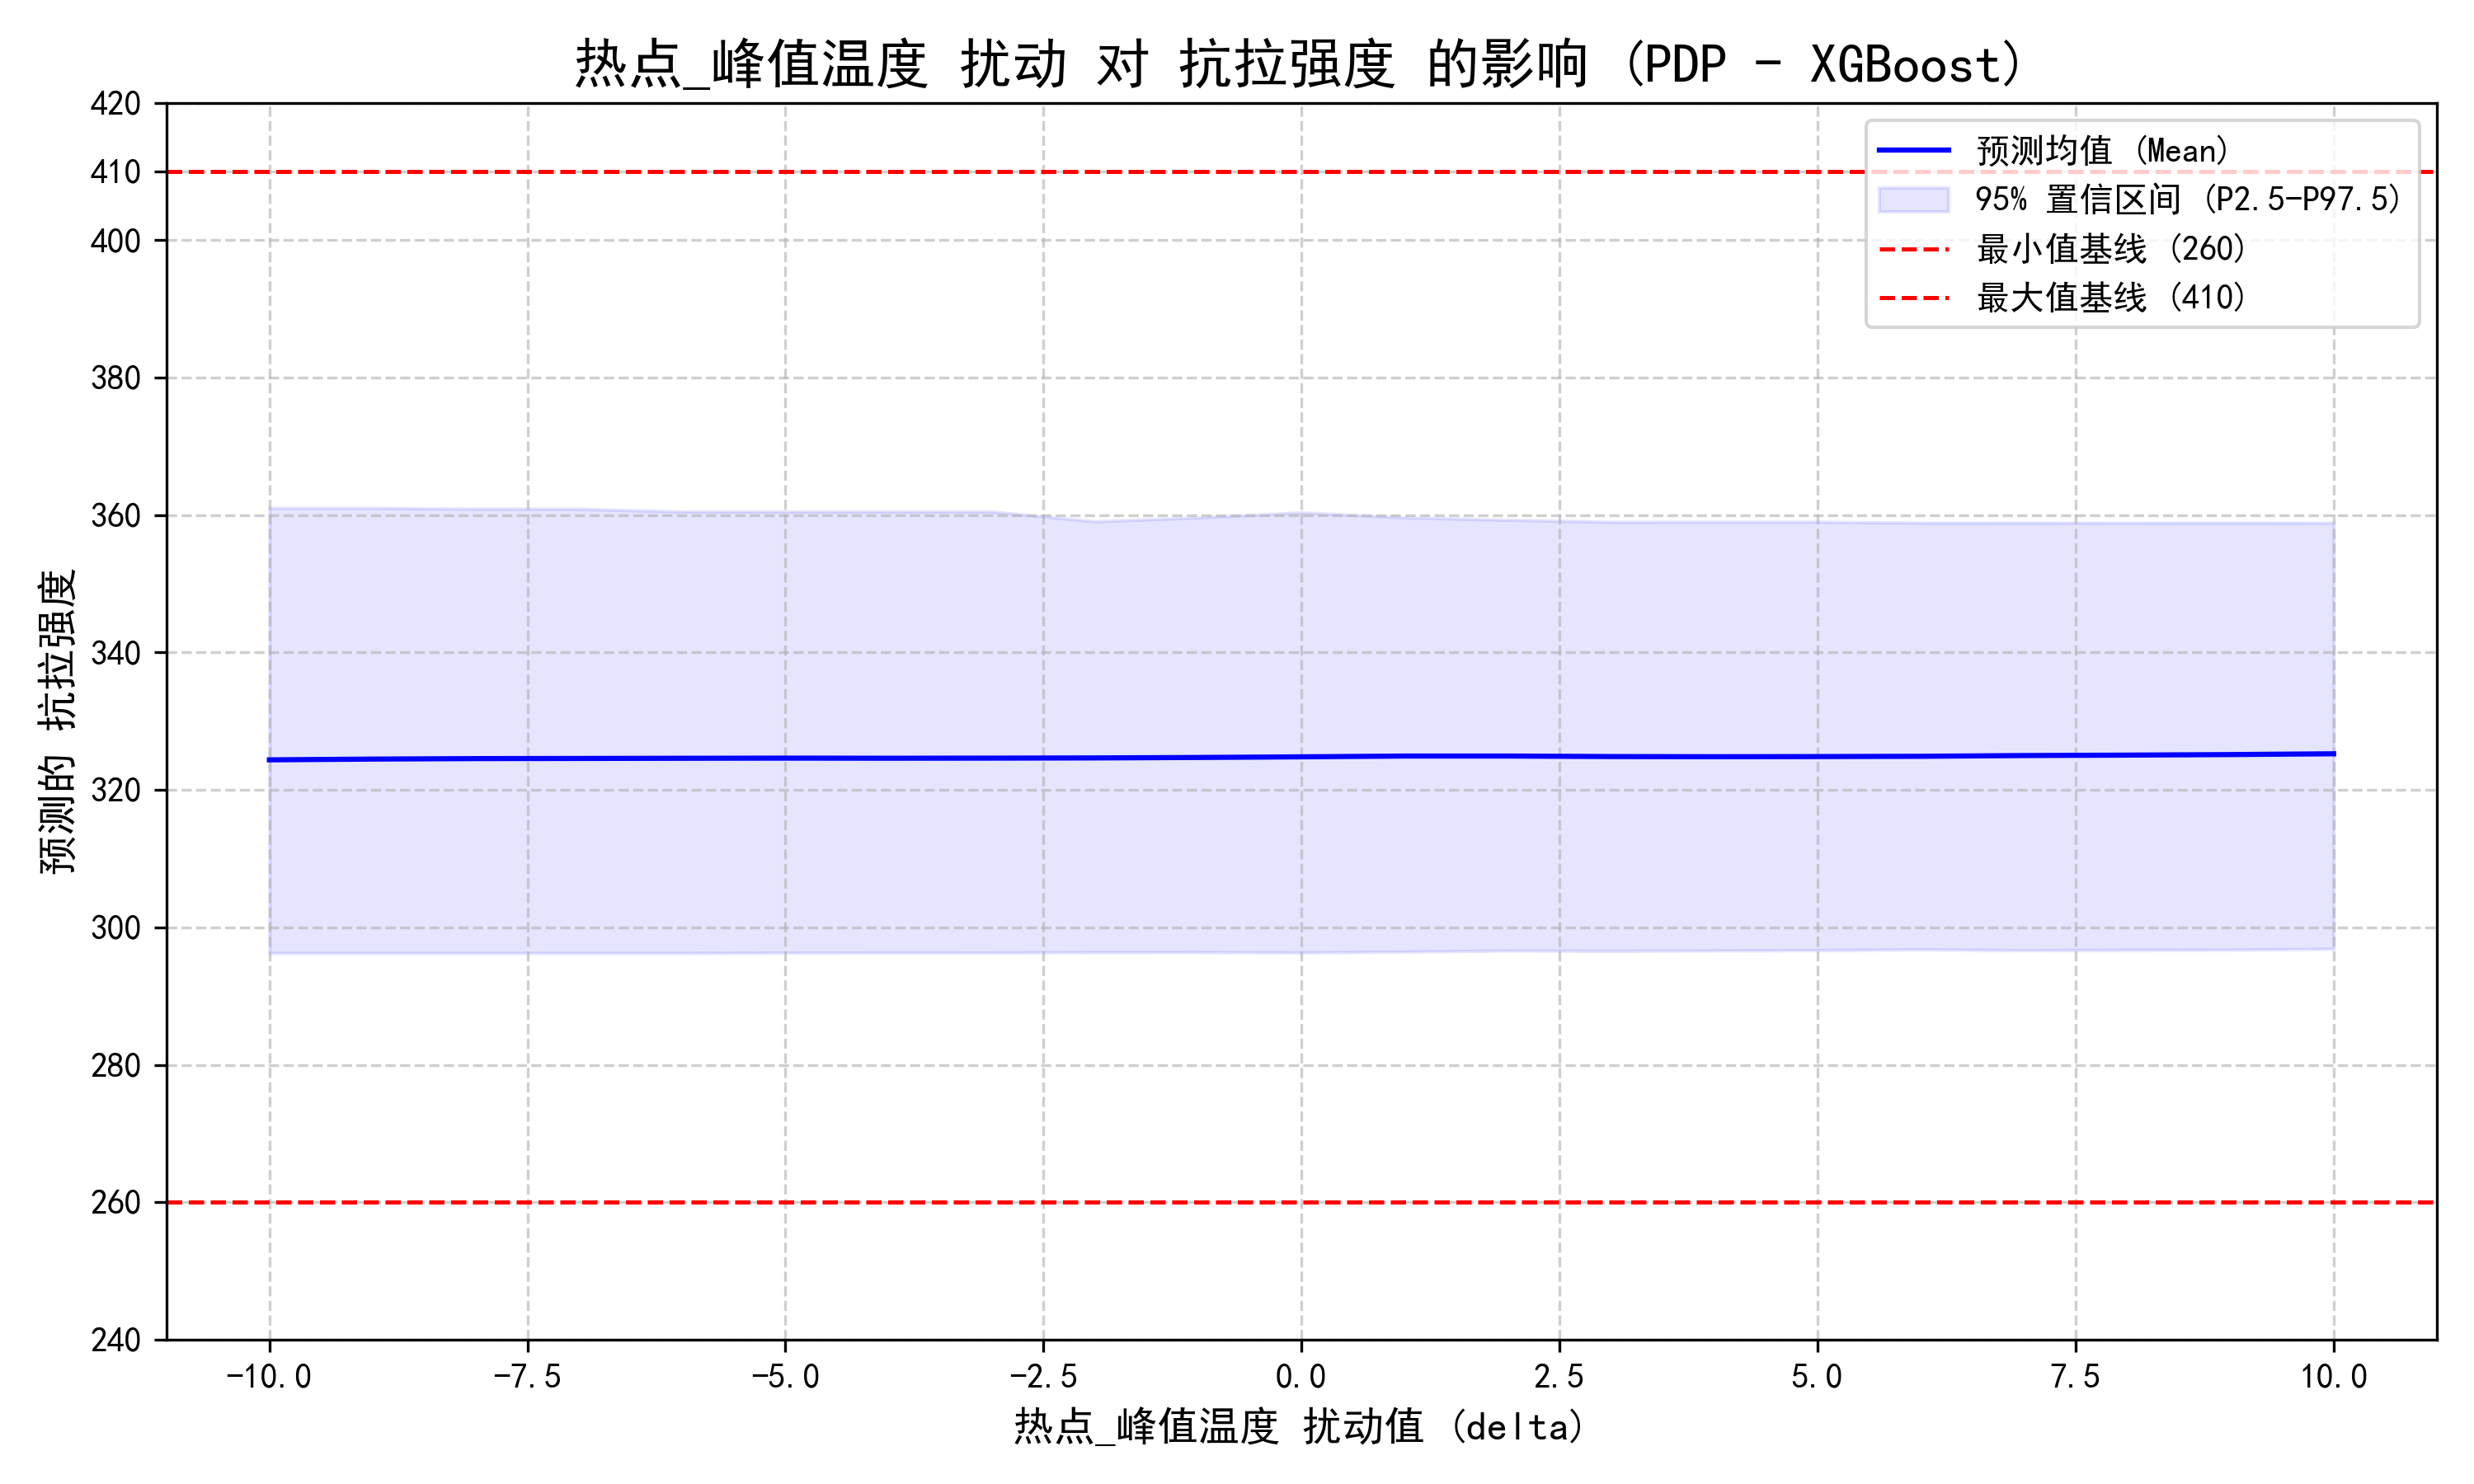
\includegraphics[width=0.75\textwidth]{fig/02b_pdp_plot_hot_spot_temp_vs_tensile_strength.png}
\caption{热点峰值温度扰动对抗拉强度影响的PDP图(基于XGBoost模型)。X轴表示热点峰值温度扰动值(delta),范围为-10.0到10.0°C;Y轴表示预测的抗拉强度,范围为240到420。蓝色实线为预测均值,浅蓝色阴影区域为95\%置信区间,红色虚线分别表示最小值基线(260)和最大值基线(410)。}
\label{fig:pdp_redian}
\end{figure}

值得注意的是,虽然PDP分析显示在较小扰动范围内(±10°C)这些参数的影响不明显,但这并不意味着这些参数在实际生产中不重要。特征重要性分析显示峰值温度和保温时长是最重要的特征之一,这表明它们对模型预测的整体贡献是显著的,但在局部小范围内变化时,影响可能被模型平均化。在实际应用中,应综合考虑特征重要性和PDP分析结果,合理设置工艺参数范围。

\subsection{模型性能总结}

综合来看,集成学习方法(特别是XGBoost)在钢铁材料性能预测任务中表现优异,主要原因包括:
\begin{enumerate}
\item \textbf{非线性建模能力}:梯度提升算法能够捕捉复杂的特征交互关系
\item \textbf{特征重要性自动学习}:自动识别对性能预测最重要的特征
\item \textbf{正则化机制}:通过L1和L2正则化防止过拟合
\item \textbf{缺失值处理}:能够自动处理数据中的缺失值
\end{enumerate}

相比之下,SVR和TabNet在本研究中表现相对较差,可能与数据规模、特征数量和超参数设置有关。但TabNet的可解释性优势使其在需要深入理解特征作用机制的场景中仍有价值。

\section{讨论}

\subsection{方法优势}

本研究的主要优势包括:
\begin{enumerate}
\item \textbf{完整的数据处理流程}:从原始时间序列数据到最终特征数据集,建立了标准化的处理流程
\item \textbf{多算法对比}:对比了5种主流机器学习算法,为实际应用提供了算法选择参考
\item \textbf{模型可解释性}:通过特征重要性和PDP分析,提供了工艺优化的具体指导
\item \textbf{实际工业数据验证}:基于真实工业生产数据,结果更具实际应用价值
\end{enumerate}

\subsection{研究局限}

研究存在以下局限:
\begin{enumerate}
\item \textbf{数据规模}:虽然处理了12,737个钢卷的原始数据,但经过去重和清洗后,最终建模样本仅2,760条,可能影响深度学习模型的性能
\item \textbf{特征维度}:仅考虑了工艺参数和化学成分,未包含微观组织信息,这可能影响断后伸长率等指标的预测精度
\item \textbf{模型泛化能力}:模型在相同工艺条件下的验证效果良好,但在不同工艺条件下的泛化能力需要进一步验证
\item \textbf{工艺优化指导}:虽然通过PDP分析揭示了参数影响趋势,但多参数联合优化的指导仍需进一步研究
\end{enumerate}

\subsection{未来研究方向}

基于本研究结果,未来可以从以下方向继续深入:
\begin{enumerate}
\item \textbf{数据扩充}:收集更多工艺条件下的数据,扩大数据集规模
\item \textbf{特征增强}:引入微观组织特征(如晶粒尺寸、相组成等)提升预测精度
\item \textbf{模型优化}:探索集成多种模型的混合预测方法,进一步提升性能
\item \textbf{在线预测}:开发实时预测系统,为生产现场提供即时性能预测
\item \textbf{工艺优化}:基于模型预测结果,开发工艺参数优化算法
\end{enumerate}

\section{结论}

本研究基于实际工业生产数据,构建了完整的AI技术应用框架用于钢铁材料性能预测。主要结论如下:

\begin{enumerate}
\item \textbf{数据驱动方法有效}:通过系统的特征工程和数据预处理,成功构建了高质量的数据集,为模型训练奠定了基础。

\item \textbf{集成学习方法优越}:XGBoost在三个性能指标上均表现最优,证明了集成学习方法在材料性能预测任务中的有效性。抗拉强度预测的R²达到0.9022,表明模型具有良好的预测能力。

\item \textbf{关键特征识别}:通过特征重要性分析,识别出峰值温度(热点和冷点)和保温时长是最重要的工艺参数,这与材料科学理论一致。

\item \textbf{工艺影响分析}:通过PDP分析,揭示了关键工艺参数对性能指标的影响趋势,为工艺优化提供了数据支持。

\item \textbf{方法可推广}:本研究建立的数据处理和建模流程可以推广到其他材料性能预测任务中,具有一定的通用性。
\end{enumerate}

本研究表明,AI技术在实际工业数据中的应用具有巨大潜力。通过合理的方法设计和模型选择,可以实现对材料性能的准确预测,为材料设计和工艺优化提供有力支持。未来随着数据规模的扩大和方法的改进,AI技术在材料科学中的应用前景将更加广阔。



\begin{thebibliography}{99}

\bibitem{chen2020}
Chen C, Ye W, Zuo Y, et al. Machine learning for materials discovery and design[J]. Annual Review of Materials Research, 2020, 50: 553-571.

\bibitem{zhang2021}
Zhang Y, Ling C. A strategy to apply machine learning to small datasets in materials science[J]. npj Computational Materials, 2021, 7(1): 1-8.

\bibitem{liu2019}
Liu R, Kumar A, Chen Z, et al. A predictive machine learning approach for microstructure optimization and materials design[J]. Scientific Reports, 2019, 9(1): 1-12.

\bibitem{wang2020}
Wang A, Liu H, Hao Y, et al. Machine learning-based prediction of steel properties using multi-source data[J]. Materials \& Design, 2020, 192: 108750.

\bibitem{chen2022}
Chen T, Guestrin C. XGBoost: A scalable tree boosting system[C]//Proceedings of the 22nd acm sigkdd international conference on knowledge discovery and data mining. 2016: 785-794.

\bibitem{ke2017}
Ke G, Meng Q, Finley T, et al. Lightgbm: A highly efficient gradient boosting decision tree[C]//Advances in neural information processing systems. 2017: 3146-3154.

\bibitem{arik2021}
Arik S O, Pfister T. TabNet: Attentive interpretable tabular learning[C]//Proceedings of the AAAI Conference on Artificial Intelligence. 2021, 35(8): 6679--6687.

\bibitem{breiman2001}
Breiman L. Random forests[J]. Machine learning, 2001, 45(1): 5-32.

\bibitem{smola2004}
Smola A J, Schölkopf B. A tutorial on support vector regression[J]. Statistics and computing, 2004, 14(3): 199-222.

\bibitem{friedman2001}
Friedman J H. Greedy function approximation: a gradient boosting machine[J]. Annals of statistics, 2001: 1189-1232.

\bibitem{agrawal2019}
Agrawal A, Choudhary A. Perspective: Materials informatics and big data: Realization of the "fourth paradigm" of science in materials science[J]. APL Materials, 2019, 7(5): 053208.

\bibitem{schmidt2019}
Schmidt J, Marques M R, Botti S, et al. Recent advances and applications of machine learning in solid-state materials science[J]. npj Computational Materials, 2019, 5(1): 1-36.

\bibitem{butler2018}
Butler K T, Davies D W, Cartwright H, et al. Machine learning for molecular and materials science[J]. Nature, 2018, 559(7715): 547-555.

\bibitem{ward2016}
Ward L, Agrawal A, Choudhary A, et al. A general-purpose machine learning framework for predicting properties of inorganic materials[J]. npj Computational Materials, 2016, 2(1): 1-7.

\bibitem{xie2018}
Xie T, Grossman J C. Crystal graph convolutional neural networks for an accurate and interpretable prediction of material properties[J]. Physical Review Letters, 2018, 120(14): 145301.

\end{thebibliography}

\end{document}

